\documentclass[11pt]{article}

\usepackage[utf8]{inputenc}
\usepackage[ngerman]{babel}
\usepackage{csquotes}

\usepackage{fullpage}
\usepackage{setspace}
\usepackage{parskip}
\usepackage{titlesec}
\usepackage{mathptmx}

\usepackage{graphicx}

\PassOptionsToPackage{
doi=false,
isbn=false,
eprint=false,
}{biblatex}
\usepackage[backend=biber]{biblatex}
\addbibresource{library.bib}

\PassOptionsToPackage{hyphens}{url}

\makeatletter

\renewenvironment{abstract}
{{\bfseries\noindent{\abstractname}\par\nobreak}\footnotesize}
{\bigskip}

\renewenvironment{quote}
  {\begin{tabular}{|p{13cm}}}
  {\end{tabular}}

\titlespacing{\section}{0pt}{*3}{*1}
\titlespacing{\subsection}{0pt}{*2}{*0.5}
\titlespacing{\subsubsection}{0pt}{*1.5}{0pt}

\usepackage{authblk}

%\usepackage{longtable}
%\usepackage{tabulary}
%\usepackage{booktabs,array,multirow}
\usepackage[colorlinks = false]{hyperref}

\begin{document}

\begin{titlepage}
   \begin{center}
       \vspace*{1cm}
       
       \Huge	
       Zusammenhang zwischen sportlichem Erfolg und Darstellung bei Wikipedia im Vergleich zwischen Sportlern und Sportlerinnen
 
       \vspace{2.0cm}
       
       
\includegraphics[width=0.4\textwidth]{logo.jpg}
 
       \vspace{1.5cm}
       \LARGE
       Josefine Busch, Lisa Hillebrand, Flip Jansen, Daniela Tumbrägel
 
       \vfill
 
       Grundlagen sozialer Netze \\
       Prof. Dr. Gefei Zhang\\
       Wintersemester 2018/2019\\
 
       \vspace{0.8cm}
      
       Hochschule für Technik und Wirtschaft\\
       Berlin\\
 
   \end{center}
\end{titlepage}



\author{Lisa Hillebrand}%
\author{Josefine Sophie Busch}%
\author{Daniela Tumbrägel}%
\author{Flip Jansen}%
\affil{HTW Berlin}%

%\date{\today}



%\begingroup
%\let\center\flushleft
%\let\endcenter\endflushleft
%\maketitle
%\endgroup

\pagebreak

\begin{abstract}
\textbf{}---%
\end{abstract}%

\section {Problemformulierung}

Die Motivation für unser Projekt ergab sich aus dem Fall von Donna Strickland, die im Jahr 2018 - zusammen mit Gérard Mourou und Arthur Ashkin - einen Nobelpreis im Bereich der Laserphysik erhalten hat \cite{nobelprize}. Sie ist die dritte Frau, der je ein Physik-Nobelpreis verliehen wurde und erst nach der Anerkennung bekam sie einen Wikipedia-Artikel (cf. Washington Post). Ihre männlichen Kollegen sind in der Online-Enzyklopädie schon seit einigen Jahren vertreten. Einige Monate zuvor wurde ein Eintrag über Strickland abgelehnt, da sie von einem der Wikipedia-Editoren als nicht wichtig genug erachtet wurde \cite{stricklandWiki}. Neben zahlreichen anderen Beispielen, zeigt dies die geschlechtsspezifische Diskriminierung auf Wikipedia und insbesondere die Ausgrenzung von Frauen in der Wissenschaft auf (cf. Guardian).

Geplant war, durch unser Projekt, numerisch und graphisch darzustellen, dass Frauen in der Wissenschaft auf Wikipedia schlechter repräsentiert werden als Männer. Bei der Suche nach effizienten Datenquellen- und -sätzen ergab sich allerdings die Problematik, dass Frauen in der Wissenschaft insgesamt so wenig vertreten sind, dass man keinen sinnvollen Vergleich zwischen Frauen und Männern herstellen kann. [TBE: Die Daten sind einfach nicht da, was ein ganz anderes gesellschaftskritisches Fass aufmacht]. 

Wir entschieden uns deshalb für einen anderen Themenbereich, in dem Frauen und Männer gleichermaßen vertreten sind: Sport. Um die Sache entsprechend einzugrenzen, wählten wir die Olympischen Sommerspiele 2016 in Rio de Janeiro. 

Im Hinblick auf die größtenteils gleichmäßige Anzahl von beiden Geschlechtern, untersuchen wir das Verhältnis von sportlichem Erfolg und der entsprechenden Darstellung auf Wikipedia. Motiviert durch die oben genannten Ereignisse, bildet sich unsere These, dass Frauen bei gleichzusetzender Leistung im Vergleich zu Männern auf Wikipedia unzureichend repräsentiert werden. Im Detail differenzieren wir dabei die mittlere Länge und die mittlere Anzahl der redaktionellen Änderungen der Wikipedia-Artikel der Sportler*innen der Olympischen Sommerspiele im Jahr 2016.

\section*{Theorie}
\label{intro}
\subsubsection*{Wikipedia}
Wikipedia wurde im Jahr 2001 gegründet \parencite{wikipediaTimeline}. Mittlerweile gibt es sprachenübergreifend über 46 Millionen Artikel \parencite{wikipedia_Size}. Von rund 35 Millionen registrierten Nutzer:innen sind jedoch nur etwa 124.000 monatlich aktiv \parencite{wikipedians}. 
Wikipedia ist zum Zeitpunkt des Verfassens dieses Texts auf dem fünften Platz der weltweit populärsten Websites \parencite{Alexa2019} und hat damit eine enorme Reichweite.
Jede Person kann zu Wikipedia beitragen und auch ohne Registrierung Artikel bearbeiten \parencite{wikipediaTutorial}. Das Erstellen neuer Artikel ist nur nach vorheriger Registrierung möglich. Jeder Artikel verfügt über eine Versionsgeschichte, in der vorherige Artikelversionen sowie die Anmerkungen der Autor:innen und Administrator:innen gespeichert werden.

\subsubsection*{Gender Bias}

Ein Bias ist eine Verzerrung bzw. ein systematischer Fehler \parencite{Wirtz}. Als Gender Bias bezeichnet man eine Bevorzugung oder Parteilichkeit gegenüber einer oder mehreren Personen ausschließlich wegen des Geschlechts. Es sollen nun einige Erkenntnisse hinsichtlich des Gender Bias im Sport zusammengefasst und und daraus die Hypothesen abgeleitet werden.

\subsubsection{Gender Bias und Wikipedia}
In mehreren Studien konnte gezeigt werden, dass ein Gender Bias sowohl in der Zusammensetzung der Autorenschaft bei Wikipedia als auch hinsichtlich der inhaltlichen Gestaltung der Artikel besteht. 
Unter den Autoren sind bestimmte Personengruppen deutlich unterrepräsentiert. In Nutzerbefragungen wurde erfasst, dass zwischen 84\% und 90\% aller Wikipidia-Autor:innen männlich sind \parencite{wikimediaReport,GraellsGarrido2015}. Hierzu muss jedoch angemerkt werden, dass die von der Wikimedia Foundation selbst durchgeführten Erhebungen Opt-in-Befragungen sind, die zu Verzerrungen führen können. So ist vorstellbar, dass weniger Frauen als Männer an der Befragung teilnehmen, sie aber eigentlich unter den Autoren deutlich häufiger vertreten sind. \textcite{Hill2013} überprüfen genau diese Kritikpunkte und berechnen einen korrigierten Wert für den Anteil Autorinnen, der jedoch auch nach Korrektur bei lediglich 16.1\% liegt. Es lässt sich also zusammenfassen, dass nach jetzigem Stand der Kenntnis deutlich weniger Frauen als Männer zu Wikipedia beitragen.

Auf inhaltlicher Ebene untersuchten verschiedene Studien das Vorliegen eines Gender Bias. \textcite{Wagner2015} analysierten Wikipedia-Artikel über bekannte Personen in vier Parametern: Abdeckungsbias (coverage bias), Strukturbias (structural bias), Lexikalischer Bias (lexical bias) und Sichtbarkeitsbias (visibility bias). Der Abdeckungsbias beschreibt, über wie viele Personen Wikipedia-Artikel bestehen. So könnte eine Annahme sein, dass über bekannte Frauen weniger Artikel verfasst werden als über bekannte Männer. Mit dem Strukturellen Bias werden Unterschiede beispielsweise in der Verlinkungsstruktur beschrieben. Ein Bias würde bestehen, wenn Frauenartikel mehr Verlinkungen auf Artikel über Männer enthalten als umgekehrt. Ein Lexikalischer Bias umfasst Unterschiede im Vokabular, mit dem Männer und Frauen beschrieben werden. Ein Beispiel für einen Bias wäre, dass in Artikeln über Frauen mehr Vokabular mit Beziehungs- oder Familienbezug verwendet wird. Der Sichtbarkeitsbias gibt an, ob es Unterschiede zwischen den Geschlechtern in der Häufigkeit gibt, mit der Artikel auf der Startseite von Wikipedia platziert werden.
In ihrer Studie konnten \textcite{Wagner2015} Evidenz für den Strukturellen und den Lexikalischen Bias finden. Artikel über Frauen verlinken häufiger auf Artikel von Männern als umgekehrt. Auf lexikalischer Ebene konnten die Autoren zeigen, dass in Artikeln über Frauen mehr Vokabular mit Bezug zu Familie und romantischen Beziehungen verwendet wird als in Artikeln über Männern. Ein Abdeckungsbias konnte nicht gezeigt werden; bekannte Frauen und Männer, die für die Studie ausgewählt wurden, waren quantitativ gleich gut vertreten.

In einer Studie von  \textcite{GraellsGarrido2015} fand sich hingegen, dass der Gender Bias auf Wikipedia mit Struktur und Inhalt von Artikeln zusammenhängt. In der Artikellänge besteht ein signifikanter Unterschied, wobei Artikel über Frauen im Mittel kürzer sind als Artikel über Männer. Die Effektstärke fiel lediglich gering aus.

Die vorliegende Untersuchung fokussiert auf den Abdeckungsbias und untersucht die Artikellänge sowie die Anzahl der Editierungen.

\subsubsection{Gender Bias im Sport}

In einigen Sportarten erhalten Sportler mehr Aufmerksamkeit als Sportlerinnen, was sich in den Umsätzen und schlussendlich auch in den Gehältern niederschlägt. So liegt das Durchschnittsgehalt in der Fußball-Bundesliga der Männer bei rund 1,5 Millionen Euro \parencite{Harris2015}, während das Durchschnittsgehalt der Frauen bei 43.000 Euro pro Jahr liegt \parencite{soccerIncomeWomen}. Zahlreiche Studien haben sich mit der Medienberichterstattung über Sportler und Sportlerinnen befasst. Zum einen gibt es Sportarten, in denen weitaus mehr Zeit der TV-Berichterstattung für die männlichen Sportler aufgewendet wird - Fußball oder Basketball sind hier nur zwei Beispiele. In der NBC-Berichterstattung über die Olympischen Spiele 2008 wurde 54,2\% der Übertragungszeit über Sportler berichtet und 44,8\% der Zeit über Sportlerinnen \parencite{Billings2008}. \textcite{Trolan2013} fassten Erkenntnisse anderer Studien zusammen und kommen zu dem Schluss, dass Frauen in der Medienberichterstattung sowohl quantitativ unterrepräsentiert sind als auch qualitativ anders berichtet wird. Die Leistungen von Frauen werden trivialisiert, indem ein stärkerer Fokus auf das Äußere von Sportlerinnen gelegt wird als auf ihre Leistungen \parencite{Harris2005,Vincent2004}. \textcite{Jones1999} untersuchten die Berichterstattung über die Olympischen Spiele 1998 und fanden, dass über Sportlerinnen mehr berichtet wird, wenn sie einer Sportart nachgehen, die als weniger maskulin beurteilt wird. \textcite{Billings2008} untersuchten, wie Sportkommentator*innen Erfolg und Misserfolg bei Sportler*innen attribuieren. Im Falle von Erfolg führten sie diesen bei Sportlern signifikant häufiger auf deren überlegene körperliche Stärke zurück.
Zusammenfassend lässt sich also sagen, dass es quantitative und qualitative Unterschiede in der Berichterstattung über Sportler und Sportlerinnen gibt. Daraus abgeleitet ergibt sich die Annahme, dass sich dies auch in der Aufmerksamkeit niederschlägt, die Sportler*innen bei Wikipedia erfahren.

\subsubsection*{Hypothesen}

Es ergeben sich folgende Hypothesen:

\textbf{Hypothese 1}. Wikipedia-Artikel über Sportler sind signifikant länger als Wikipedia-Artikel über Sportlerinnen.

\textbf{Hypothese 2}. Wikipedia-Artikel über Sportler wurden signifikant häufiger editiert als Wikipedia-Artikel über Sportlerinnen.

Diese Untersuchung überprüft die Hypothesen anhand von acht ausgewählten Wettkämpfen bei den Olympischen Spielen in Rio 2016.

\section{Methodik // Busch, Josefine 560106}
\label{igw}

\subsection{Erhebungsart}
Zur Beschaffung der Daten stehen uns zwei Möglichkeiten zur Verfügung. Auf der offiziellen Webseite der Olympischen Kommission sind die Namen der Teilnehmenden der vergangenen Spiele veröffentlicht \parencite{olympicResults}. Der Vorteil dieser Daten ist, dass sie bereits in weibliche und männliche Teilnehmer*innen unterteilt sind. Alternativ sind auch direkt auf Wikipedia Listen der Teilnehmenden zu finden. \parencite{WikpediaOlympics2016} Diese Listen beinhalten direkte Verlinkungen zu den jeweiligen Seiten der Sportler*innen. Allerdings ist hier nicht mehr ohne Weiteres auszulesen, welchem Gender die Person angehört. Um diese Information zu bekommen müsste der Fließtext auf die verwendeten Pronomen untersucht werden. Auch andere Informationen sind bei Wikipedia nicht mehr so leicht auslesbar wie aus der Liste von \textit{olympic.org}. Besonders sind die Sportler*innen nach dem Alphabet geordnet nicht nach dem erreichten Rang, dieser müsste also ebenfalls aus dem Fließtext ausgelesen werden.

Die Liste der Olympischen Spiele 2016 von \textit{olympic.org} enthält strukturierte Daten von denen uns speziell nur die Spalten "Sport", "Discipline", "Event", "Names" und "Gender" interessieren.
Die Länge der Artikel, gemessen an der Anzahl der Wörter, und die Anzahl der Editierungen der einzelnen Artikel müssen erst berechnet beziehungsweise von Wikipedia direkt abgefragt werden. Diese Daten liegen in unstrukturierter Form vor.

\subsection{Stichproben}
Da nicht in allen Sportarten Frauen und Männer in vergleichbaren Disziplinen antreten und in manchen Disziplinen Teams gegeneinander antreten, wählen wir 8 Disziplinen aus unterschiedlichen Sportarten aus, welche unsere Anforderungen erfüllen. Die Anforderungen sind, dass die Disziplinen für Frauen und Männer gleich sind bzw. gleich bezeichnet sind und dass sie keine Teamdisziplinen sind.

Die ausgewählten Disziplinen sind:
\begin{itemize}
\item Turmspringen 10m
\item Bogenschießen Einzelwettkampf
\item Fechten Épée Einzelwettkampf
\item Moderner Fünfkampf Einzelwettkampf
\item Leichtathletik Stabhochsprung
\item Schwimmen 100m Freistil
\item Radsport Straße Einzelwettkampf
\item Leichtathletik Sprint 100m
\end{itemize}

Um die Artikel von Wikipedia zu bekommen und von diesen die Länge in Wörtern verwenden wir ein Modul von GitHub Benutzer Jonathan Goldsmith \parencite{GoldsmithWikipedia}. Mit diesem Modul und den Titeln der Wikipedia-Seiten können die Artikel abgerufen werden. Danach muss nur noch die Anzahl der Wörter ermittelt werden. Mit Stichproben soll geprüft werden, dass die korrekten Artikel zurückgegeben und gezählt werden.

Für die Zwischenspeicherung der Daten im Jupyter Notebook verwenden wir \textit{pandas} Dataframes. Außerhalb des Programms sind die Daten in CSV-Dateien abgelegt. Für die grafische Darstellung im Notebook verwenden wir außerdem \textit{matplotlib.pyplot} und \textit{seaborn}.

\subsection{Auswertungsmethoden}
Für die Darstellung und Auswertung der Daten unterscheiden wir nach Gender der Sporler*innen und den Disziplinen.

\subsubsection{Verteilung der Daten}
Um ein besseres Verständnis für unsere Daten zu entwickeln wollen wir uns diese zunächst in einem Histogramm anschauen. Das Histogramm trägt auf der X-Achse die Anzahl der Wörter beziehungsweise Editierungen auf und auf der Y-Achse die Häufigkeit, mit der die jeweilige Anzahl vorkam. Dies soll uns zeigen wie die Daten verteilt sind und ob eine Normalverteilung vorliegt.

Mit weiteren Balkendiagrammen wollen wir die Extrem-, Mittel- und Medianwerte darstellen.

\subsubsection{Ausreißer}
Wir gehen davon aus, dass wir einige Ausreißer in unseren Daten haben werden. Sportler wie beispielsweise Usain Bolt werden erwartbar vergleichsweise lange Wikipedia-Artikel aufweisen. Um einen besseren Überblick über die Anzahl und Verteilung der Ausreißer zu bekommen, werden wir die Daten in einem Boxplot und einem Stripplot darstellen. Der Boxplot zeigt außerdem die Quantile. Als Ausreißer werden alle Datenpunkte im Boxplot dargestellt, die außerhalb des Bereiches liegen, in dem 90\% der Daten zu finden sind.

\subsubsection{Signifikanz}
Sollten unsere Daten normalverteilt sein, werden wir die Signifikanz mit Hilfe des T-Tests untersuchen, andernfalls wollen wir den Mann-Whitney-U-Test verwenden. 

"The Mann-Whitney U test is used to compare differences between two independent groups when the dependent variable is either ordinal or continuous, but not normally distributed." \parencite{LundResearchLtd}


\section {Durchführung // Jansen, Flip 558059}
Ausgehend von der Wikipedia-Überblicksseite \cite{wikiOlympicComp}haben wir rekursiv alle Sportarten sowie auf der untersten Ebene die Links der einzelnen Sportler*innen einer Sportart auf Wikipedia gesammelt und in eine CSV-Datei geschrieben. 

Um mögliche Fehlern beim Sammeln der Daten von der Olympic.org - Seite zu vermeiden, haben wir das Olympic Studies Centre angeschrieben, die uns eine Excel-Tabelle mit den ausführlichen Ergebnissen der Olympischen Sommerspiele 2016 zur Verfügung gestellt haben.

Um die Wikipedia-Links mit den von uns benötigten Daten der Ergebnistabelle zu verbinden, mussten wir die unterschiedlichen Namensformate anpassen und Sonderzeichen umwandeln. So setzt zum Beispiel Wikipedia bei Namensgleichheit von in Wikipedia erfassten Personen eine Kategoriebezeichnung ans Ende des Namens: "(diver)".

Trotzdem konnten wir einige Links nicht automatisiert zuordnen, da es zum einen in den Ergebnistabelle Rechtschreibfehler in den Namen gibt, zum anderen, weil gerade bei Namen aus Sprachgebieten mit nicht-lateinischer Schrift unterschiedliche !!!Konvertierungen!!!

\section {Ergebnisse}
\subsection{Anzahl der Editierungen // Tumbrägel, Daniela 558529}
\subsubsection{Verteilung}
Wie bei der Anzahl der Wörter im zuvorkommenden Abschnitt fällt bei der Betrachtung des Histogramms auf, dass es sich nicht um eine Normalverteilung handelt.

Da die Histogramme der verschiedenen Disziplinen sehr linksbündig sind, wird diese Beobachtung dadurch zusätzlich bestätigt. 

Die folgenden Grafiken zeigen jeweils die Maximal-, Mittel- und Medianwerte sowie die Standardabweichung der Editierungen pro Disziplin. 

Mit Blick auf die Maxima der Editierungen per Disziplin ist erkennbar, dass es durchaus Unterschiede zwischen Frauen und Männern gibt, da insbesondere in den Disziplinen "Turmspringen 10m", "Radsport Straße Einzelwettkampf" und "Leichtathletik Sprint 100m" signifikante Unterschiede zugunsten der Männer sichtbar sind. Allerdings ist dies nur bedingt aussagekräftig, da es sich bei den Maxima um Ausreißer handeln kann, die nicht maßgeblich für die durchschnittliche Verteilung sind. Dies verifizieren wir durch nachfolgende Plots (s. Figure 10).

Das Histogramm, dass den Mittelwert aufführt, zeigt ähnliche Beobachtungen, die jedoch ebenfalls aufgrund von Ausreißern schwer zu interpretieren sind.

Grundsätzlich kann aber festgehalten werden, dass sehr markante Extremwerte primär bei den Männern - mit einem Spitzenwert von 3276 Editierungen - zu finden sind.

Aufgrund der Verteilung der Daten ist der Median hingegen durch die Sortierung der Ergebnisse vergleichsweise aussagekräftig. Dieser visualisiert hier, dass es nur in der Disziplin "Radsport Straße Einzelwettkampf" signifikante Unterschiede bei Frauen und Männern bzgl. der Editierungen der Wikipedia-Artikel gibt.

\begin{table}
\begin{tabular}{ c|c|c|c|c }
  Disziplin & Maximum & Mittelwert & Median & Standard Abweichung \\
  \hline
  Turmspringen 10m & 405 & 74.535714 & 40.5 & 275.561111 \\
  Bogenschießen Einzelwettkampf & 321 & 38.171875 & 26.0 & 225.399046 \\
  Fechten Épée Einzelwettkampf & 204 & 43.297297 & 30.0 & 689.748088 \\
  Moderner Fünfkampf Einzelwettkampf & 107 & 28.916667 & 18.5 & 148.771754 \\
  Leichtathletik Stabhochsprung & 396 & 83.281250 & 49.0 & 424.061838\\
  Schwimmen 100m Freistil & 521 & 109.333333 & 47.0 & 533.158020\\
  Radsport Straße Einzelwettkampf & 557 & 148.066667 & 97.0 & 984.240138\\
  Leichtathletik Sprint 100m & 710 & 67.675000 & 41.0 & 487.333815\\
\end{tabular}
\caption{\label{tab:table-name}Kennwerte Frauen}
\end{table}

\begin{table}
\begin{tabular}{ c|c|c|c|c }
  Disziplin & Maximum & Mittelwert & Median & Standard Abweichung \\
  \hline
  Turmspringen 10m & 2796 & 152.250000 & 33.5 & 961.725893 \\
  Bogenschießen Einzelwettkampf & 211 & 38.593750 & 26.0 & 136.328090\\
  Fechten Épée Einzelwettkampf & 138 & 35.297297 & 30.0 & 188.961311 \\
  Moderner Fünfkampf Einzelwettkampf & 58 & 20.000000 & 13.0 & 139.773521\\
  Leichtathletik Stabhochsprung & 621 & 68.687500 & 32.5 & 505.014347\\
  Schwimmen 100m Freistil & 945 & 120.937500 & 44.5 & 564.130686\\
  Radsport Straße Einzelwettkampf & 2466 & 407.166667 & 233.5 & 1882.713246\\
  Leichtathletik Sprint 100m & 3277 & 161.387500 & 54.0 & 1262.914988\\
\end{tabular}
\caption{\label{tab:table-name}Kennwerte Männer}
\end{table}

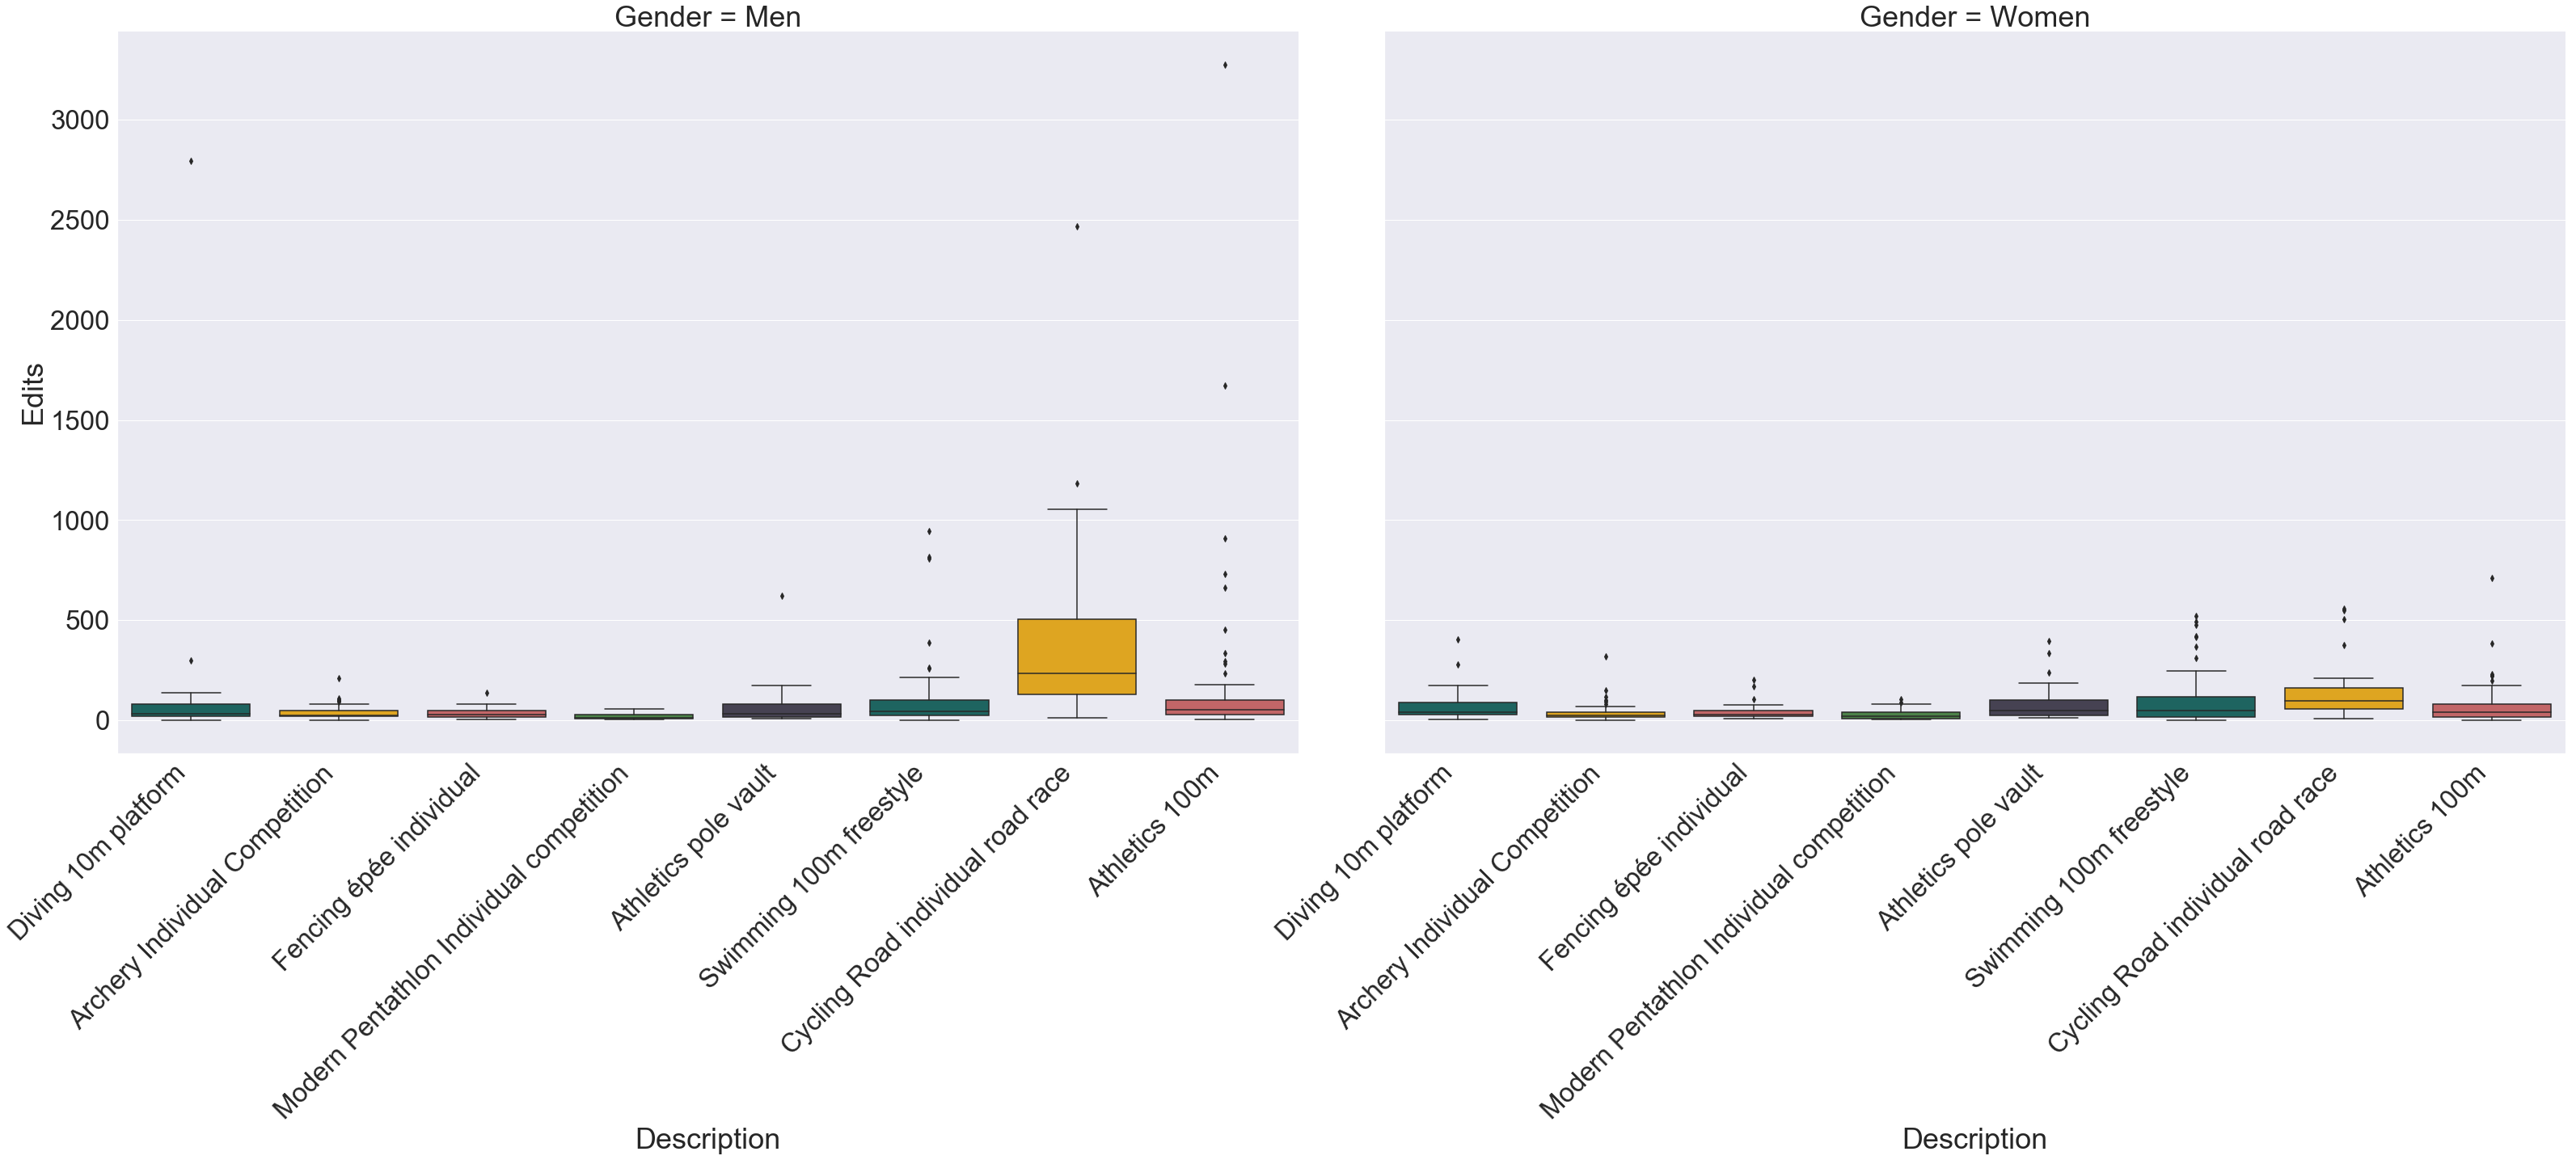
\includegraphics[width=1\textwidth]{figures/editcount_boxplot.png}

\subsubsection{Ausreißer}
Wie in der Methodik beschrieben, nutzen wir Box- und Stripplots insbesondere zur Visualisierung der Ausreißer in der vorhandenen Datenquelle. Die Abbildungen zeigen jeweils die Männer auf der linken und die Frauen auf der rechten Seite. 

Es ist deutlich erkennbar, dass bei den Männern mehrere sehr hohe Werte aufzufinden sind während es bei den Frauen zwar ebenfalls viele Ausreißer gibt, diese allerdings vergleichsweise niedrig angesiedelt sind. Die Disziplinen "Turmspringen 10m", "Radsport Straße Einzelwettkampf" und  "Leichtathletik Sprint 100m" fallen bei den Männern durch vereinzelte hochwertige Ergebnisse besonders auf. Bei den Frauen ist nur ein vergleichsweise hochwertiger Ausreißer in der Disziplin "Leichtathletik Sprint 100m" zu erkennen, der sich allerdings nur marginal von den restlichen Ausreißern abgrenzt. 

\subsubsection{Signifikanz}

Der Mann-Whitney-U-Test zeigt mit Hilfe der Berechnung des P-Wertes, wie oben bei den Medianwerten bereits angedeutet, dass es größtenteils keine signifikanten Unterschiede zwischen Frauen und Männern gibt. Wie bei der Anzahl der Wörter ist auch bei der Anzahl der Editierungen in 7 von 8 Disziplinen keine Signifikanz zu erkennen.

\begin{tabular}{ c|c|c }
  Disziplin & P-Value & Signifikanz \\
  \hline
  Turmspringen 10m & 0.222952 & nicht signifikant \\
  Bogenschießen Einzelwettkampf & 0.283641 & nicht signifikant \\
  Fechten Épée Einzelwettkampf & 0.229373 & nicht signifikant \\
  Moderner Fünfkampf Einzelwettkampf & 0.095515 & nicht signifikant \\
  Leichtathletik Stabhochsprung & 0.085362 & nicht signifikant \\
  Schwimmen 100m Freistil & 0.448976 & nicht signifikant \\
  Radsport Straße Einzelwettkampf & 0.000242 & signifikant \\
  Leichtathletik Sprint 100m & 0.013091 & signifikant \\
\end{tabular}

Die zweite Hypothese ist somit ebenfalls widerlegt. 


\section {Diskussion}

\printbibliography
\end{document}

